\documentclass[tikz,border=5pt]{standalone}
\usepackage{amsmath,amssymb}
\begin{document}
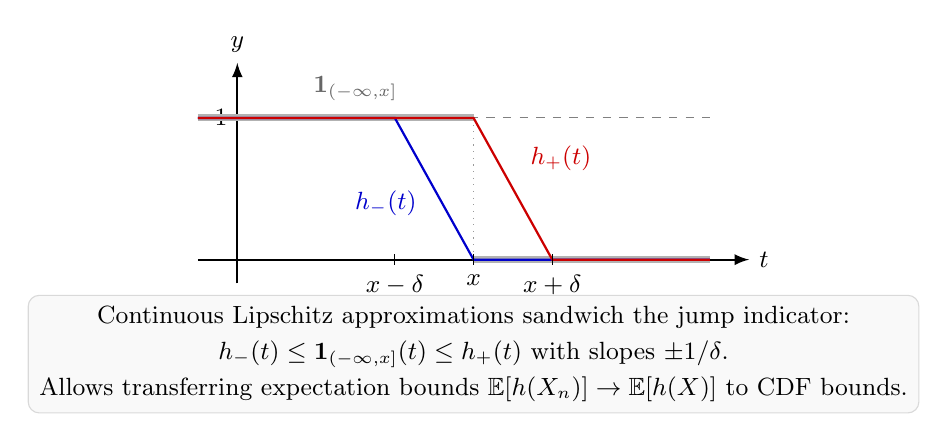
\begin{tikzpicture}[>=latex, font=\small]
  \draw[->, thick] (-0.5, 0) -- (6.5, 0) node[right] {$t$};
  \draw[->, thick] (0, -0.3) -- (0, 2.5) node[above] {$y$};

  \node[left] at (0, 1.8) {$1$};
  \draw[dashed, gray] (0, 1.8) -- (6, 1.8);

  % Indicator function 1_{(-\infty, x]}
  \draw[line width=2.5pt, gray!60] (-0.5, 1.8) -- (3, 1.8);
  \draw[line width=2.5pt, gray!60] (3, 0) -- (6, 0);
  \draw[dotted, gray!80] (3, 1.8) -- (3, 0);
  \node[above, gray!80!black] at (1.5, 1.9) {$\mathbf{1}_{(-\infty, x]}$};

  % h_-(t) lower bound
  \draw[thick, blue!80!black] (-0.5, 1.8) -- (2.0, 1.8) -- (3.0, 0) -- (6.0, 0);
  \node[blue!80!black, below left] at (2.4, 1.0) {$h_-(t)$};

  % h_+(t) upper bound
  \draw[thick, red!80!black] (-0.5, 1.8) -- (3.0, 1.8) -- (4.0, 0) -- (6.0, 0);
  \node[red!80!black, above right] at (3.6, 1.0) {$h_+(t)$};

  \foreach \x/\lbl in {2.0/x-\delta, 3.0/x, 4.0/x+\delta} {
    \draw (\x, 2pt) -- (\x, -2pt) node[below] {$\lbl$};
  }

  \node[align=center, fill=gray!5, draw=gray!30, rounded corners, inner sep=4pt] at (3.0, -1.2)
    {Continuous Lipschitz approximations sandwich the jump indicator:\\[2pt]
     $h_-(t) \le \mathbf{1}_{(-\infty, x]}(t) \le h_+(t)$ with slopes $\pm 1/\delta$.\\[2pt]
     Allows transferring expectation bounds $\mathbb{E}[h(X_n)] \to \mathbb{E}[h(X)]$ to CDF bounds.};
\end{tikzpicture}
\end{document}
